\documentclass{article}
\usepackage[paperwidth=145mm, paperheight=120mm, margin=3mm]{geometry}
\usepackage{tikz}
\usepackage{amsmath}
\usepackage{amssymb}
\usetikzlibrary{positioning, shapes.geometric, arrows.meta, fit, backgrounds, calc}
\pagestyle{empty}

\definecolor{procboxblue}{HTML}{1F6FB2}
\definecolor{procboxbg}{HTML}{E8F1FA}
\definecolor{loopgrey}{HTML}{555555}
\definecolor{loopbg}{HTML}{F4F4F4}

\begin{document}
\noindent\hspace*{-2mm}%
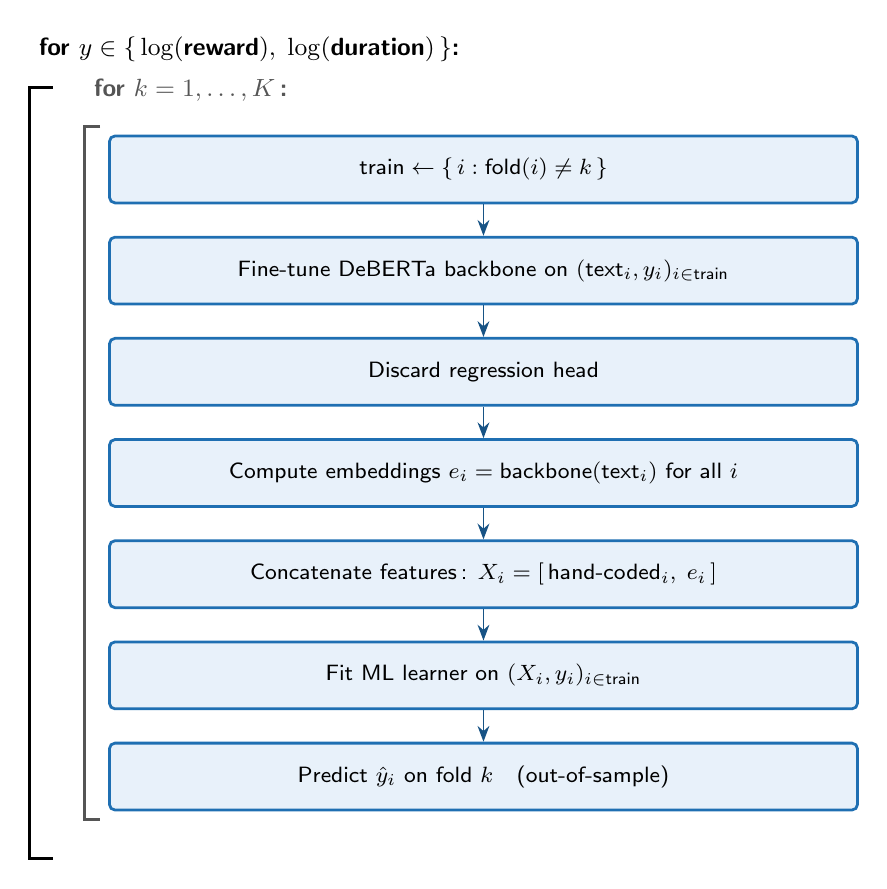
\begin{tikzpicture}[
  font=\sffamily\footnotesize,
  node distance=4mm,
  procbox/.style={
    draw=procboxblue,
    line width=1pt,
    fill=procboxbg,
    rectangle,
    rounded corners=2pt,
    minimum width=95mm,
    minimum height=8.5mm,
    align=center,
    inner sep=4pt,
    text=black
  }
]

  % --- Steps stacked top-down ---
  \node[procbox]              (s1) {$\text{train} \leftarrow \{\,i : \text{fold}(i) \neq k\,\}$};
  \node[procbox, below=of s1] (s2) {Fine-tune DeBERTa backbone on $(\text{text}_i, y_i)_{i \in \text{train}}$};
  \node[procbox, below=of s2] (s3) {Discard regression head};
  \node[procbox, below=of s3] (s4) {Compute embeddings $e_i = \text{backbone}(\text{text}_i)$ for all $i$};
  \node[procbox, below=of s4] (s5) {Concatenate features\,: $X_i = [\,\text{hand-coded}_i,\; e_i\,]$};
  \node[procbox, below=of s5] (s6) {Fit ML learner on $(X_i, y_i)_{i \in \text{train}}$};
  \node[procbox, below=of s6] (s7) {Predict $\hat{y}_i$ on fold $k$\quad(out-of-sample)};

  % Arrows between procboxs
  \foreach \a/\b in {s1/s2, s2/s3, s3/s4, s4/s5, s5/s6, s6/s7}
    \draw[-Stealth, line width=0.6pt, color=procboxblue!75!black] (\a) -- (\b);

  % --- Inner-loop bracket (left side) and label ---
  \coordinate (top)    at ($(s1.north west)+(-3mm,1mm)$);
  \coordinate (bottom) at ($(s7.south west)+(-3mm,-1mm)$);
  \draw[loopgrey, line width=1pt]
       (top) ++(2mm,0) -- (top) -- (bottom) -- ++(2mm,0);
  \node[loopgrey, anchor=south west, font=\sffamily\bfseries\small]
       at ([yshift=2mm]top) {for $k = 1, \ldots, K$\,:};

  % --- Outer-loop bracket (further left) and label ---
  \coordinate (otop)    at ($(top)+(-7mm,5mm)$);
  \coordinate (obottom) at ($(bottom)+(-7mm,-5mm)$);
  \draw[black, line width=1.2pt]
       (otop) ++(3mm,0) -- (otop) -- (obottom) -- ++(3mm,0);
  \node[black, anchor=south west, font=\sffamily\bfseries\small]
       at ([yshift=2mm]otop) {for $y \in \{\,\log(\text{reward}),\;\log(\text{duration})\,\}$:};

\end{tikzpicture}
\end{document}
